% !TEX root = ../../main.tex

\subsection{Predicting multicomponent adsorption}

Until now, we have only referred to isotherms pertaining to the adsorption
of a single adsorbate. However, besides gas storage, most if not all
industrial applications of adsorbents involve multiple chemical 
species undergoing competitive adsorption. Experiments involving
several adsorbents are generally difficult and time consuming.
There is therefore a requirement to predict such multicomponent systems
in order to rapidly screen for potentially interesting separations
starting from pure component data.

To this end, the several methods have been devised, with perhaps
the most common approach as considering the adsorbed phase as 
an analogue to a fluid mixture. This method, also known as the 
ideal adsorbed solution theory (IAST), has been implemented in
pyGAPS and will be presented here. Other multicomponent theories
such as real adsorbed solution theory (RAST) or the Nitta model
exist but usually require more information about specific
surface binary activity coefficients to be well suited to a
general high throughput approach.

\subsubsection{Ideal adsorbed solution theory}

The \texttt{pyGAPS} framework includes a modified version of 
the pyIAST code~\cite{simonPyIASTIdealAdsorbed2016} which has 
been adapted to work with the \texttt{Isotherm} 
classes. Both model isotherms and real data can be used for 
IAST, with spreading pressure being calculated through the 
underlying isotherm model or through interpolation, respectively. 

In this case, we fit the experimental data to the available models 
in \texttt{pyGAPS} which have been presented in Section~\ref{pyg:models},
then use the resulting model isotherms for IAST simulations. 
In order to get a `best-fit' model isotherm,
we use the function in Listing~\ref{lst:model},
which fits all available models and selects the one with the lowest 
residuals between the fitted function and the real data.
The isotherms and their best-fitting model is displayed in 
Figure~\ref{pyg:fig:takedaco2n2iso} for the \ce{CO2}-\ce{N2} pair and 
in Figure~\ref{pyg:fig:takedac3h6c3h8iso} for the \ce{C3H8}-\ce{C3H6} pair.

\begin{python}[caption={Guessing the best model},label={lst:model}]
model = pygaps.ModelIsotherm.from_pointisotherm(iso, guess_model=True)
\end{python}
\begin{pythonout}
Attempting to model using Henry
Model Henry success, rmse is 7.42
Attempting to model using Jensen-Seaton
Modelling using Jensen-Seaton failed
...............................
Best model fit is Quadratic
\end{pythonout}

For the carbon dioxide separation, we simulate all equilibrium 
points for the adsorbed and gaseous phases at different concentrations 
of the two gases at 1 bar. To do this we use the \inline{pygaps.iast_vle()}
function which produces an analogue of a vapour-liquid equilibrium at 
a specified pressure for a binary mixture. The resulting graph of this
function can be seen in Figure~\ref{pyg:fig:takedac3h6c3h8iast}.
As expected, the predicted adsorbed mixture is rich in carbon dioxide.
Selectivity can also be calculated in a single point, with the value at 
15\% \ce{CO2} and \SI{1}{bar} being 16.5. 

\begin{figure}[htb]

    \centering
    \begin{subfigure}[b]{.5\textwidth}
        \centering
        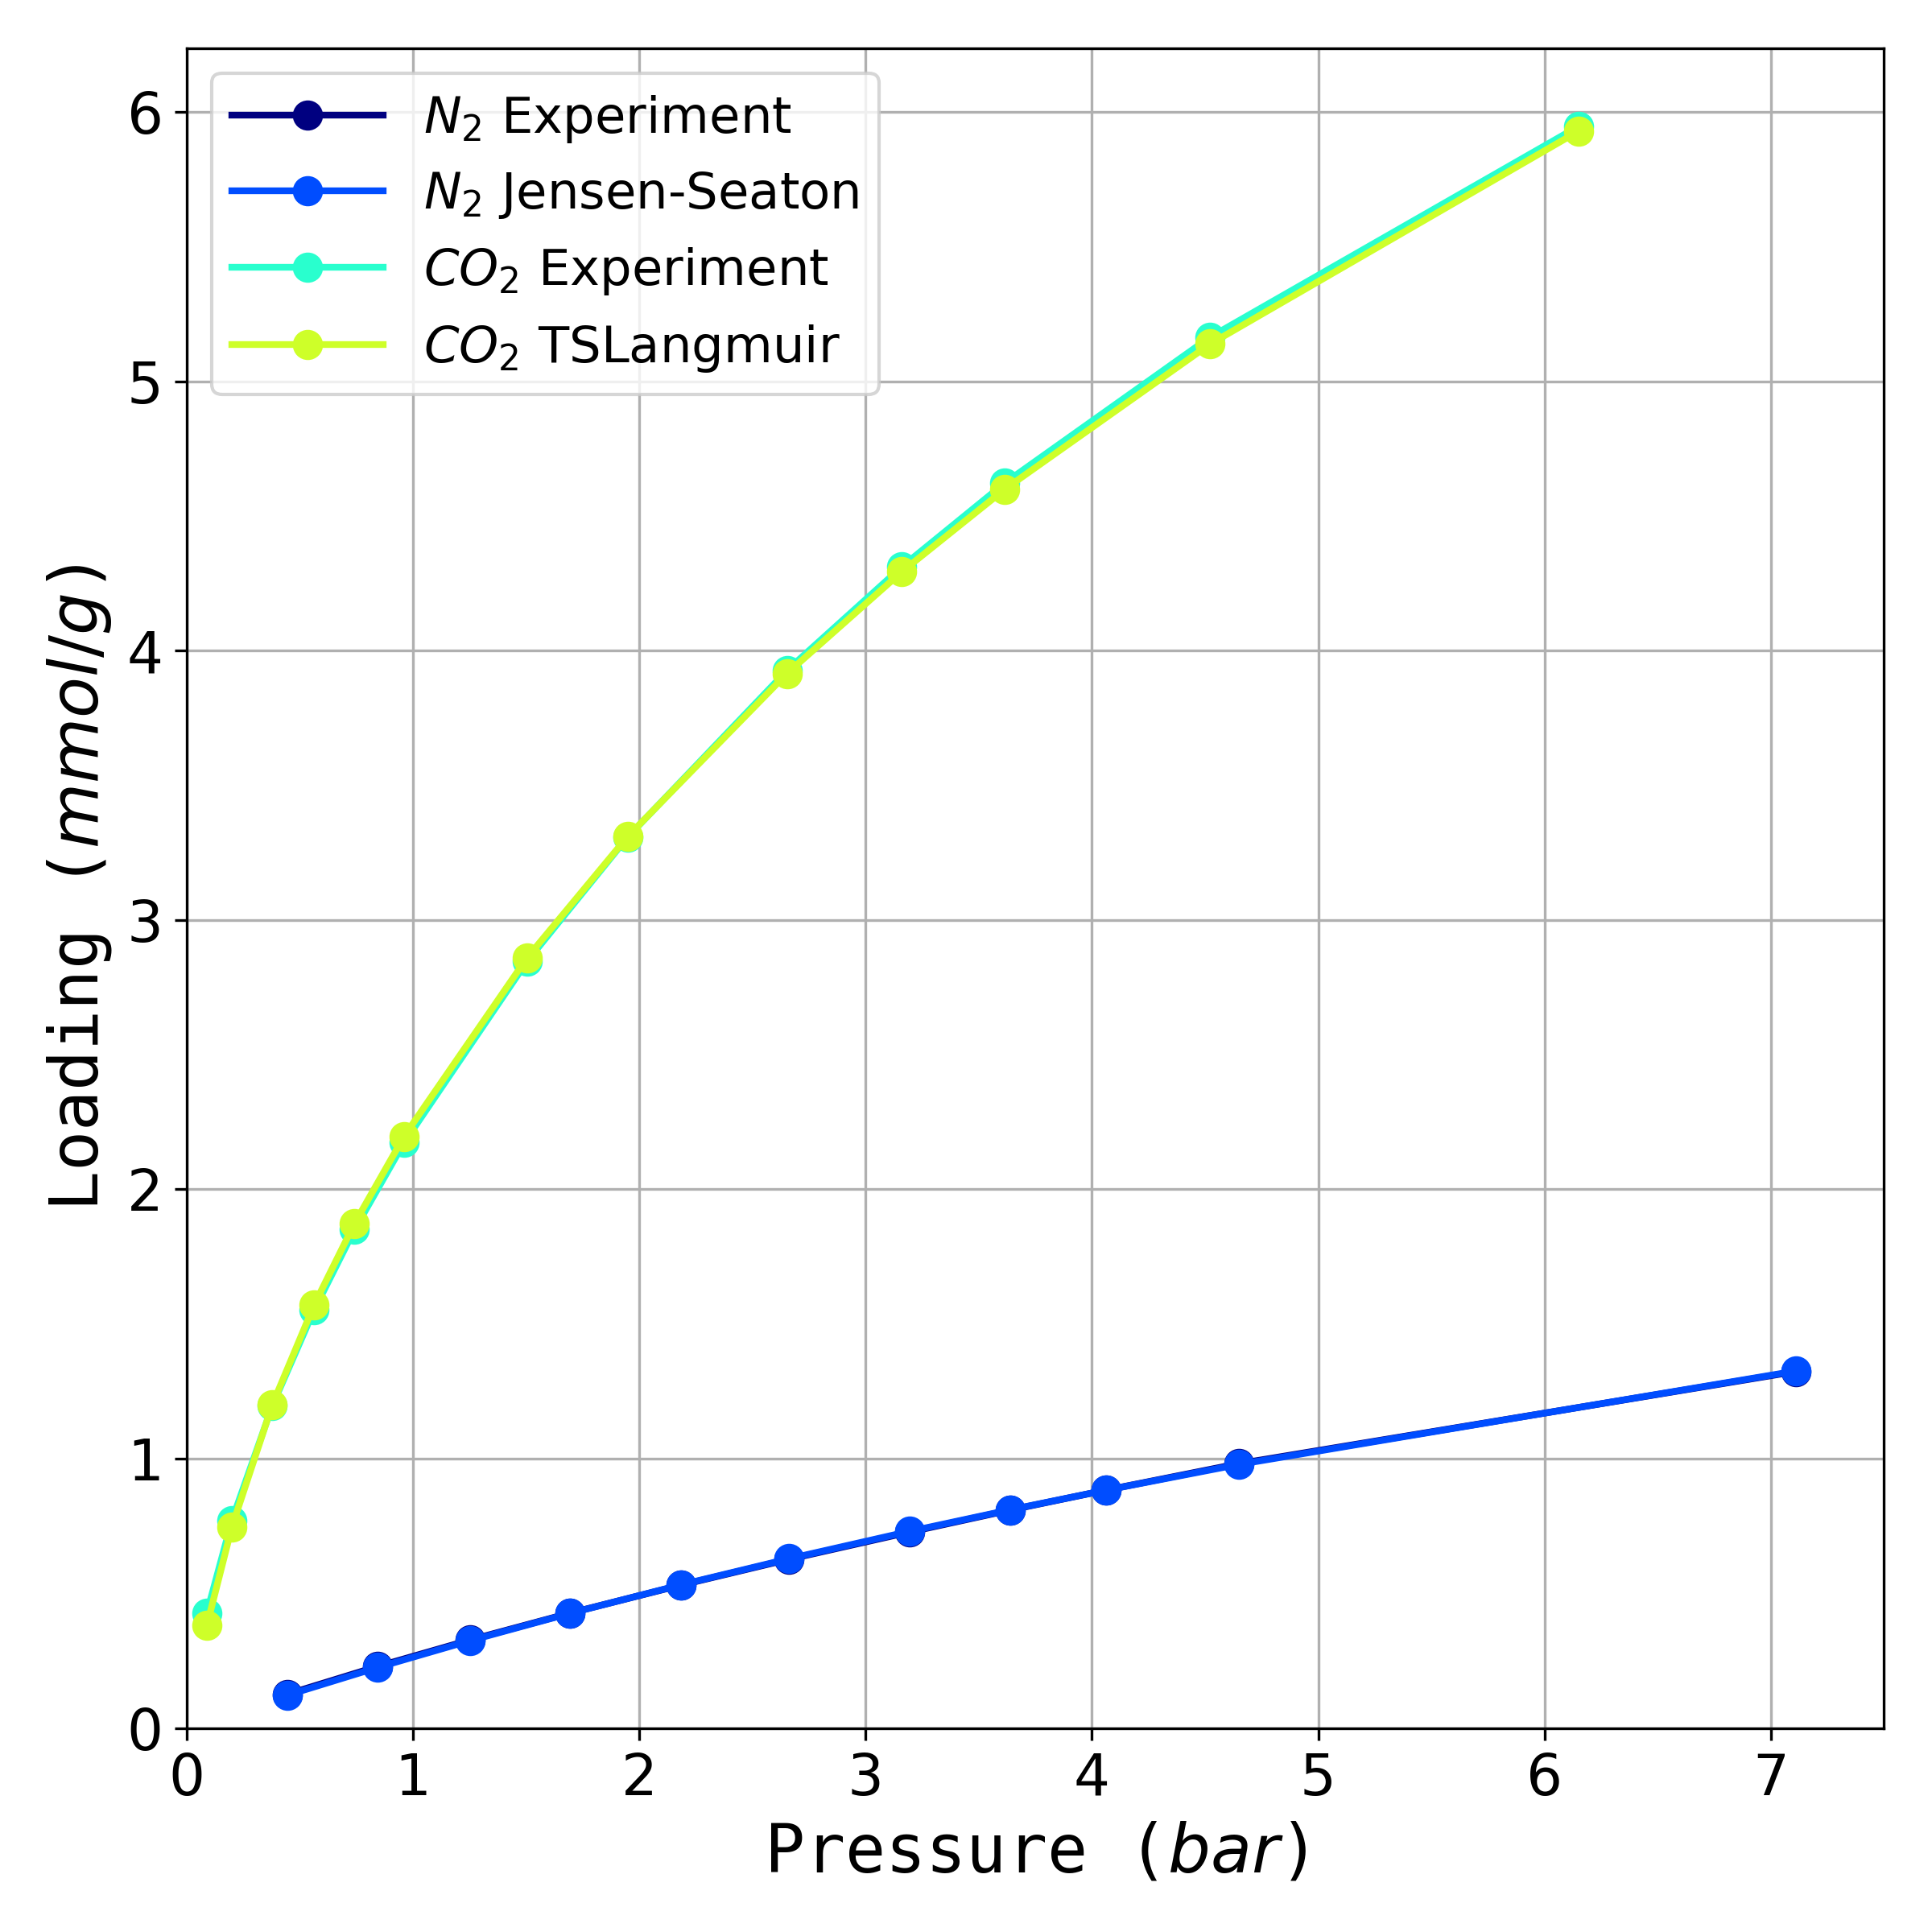
\includegraphics[width=.8\linewidth]{iast/takeda-co2n2}
        \caption{}%
        \label{pyg:fig:takedaco2n2iso}
    \end{subfigure}%
    \begin{subfigure}[b]{.5\textwidth}
        \centering
        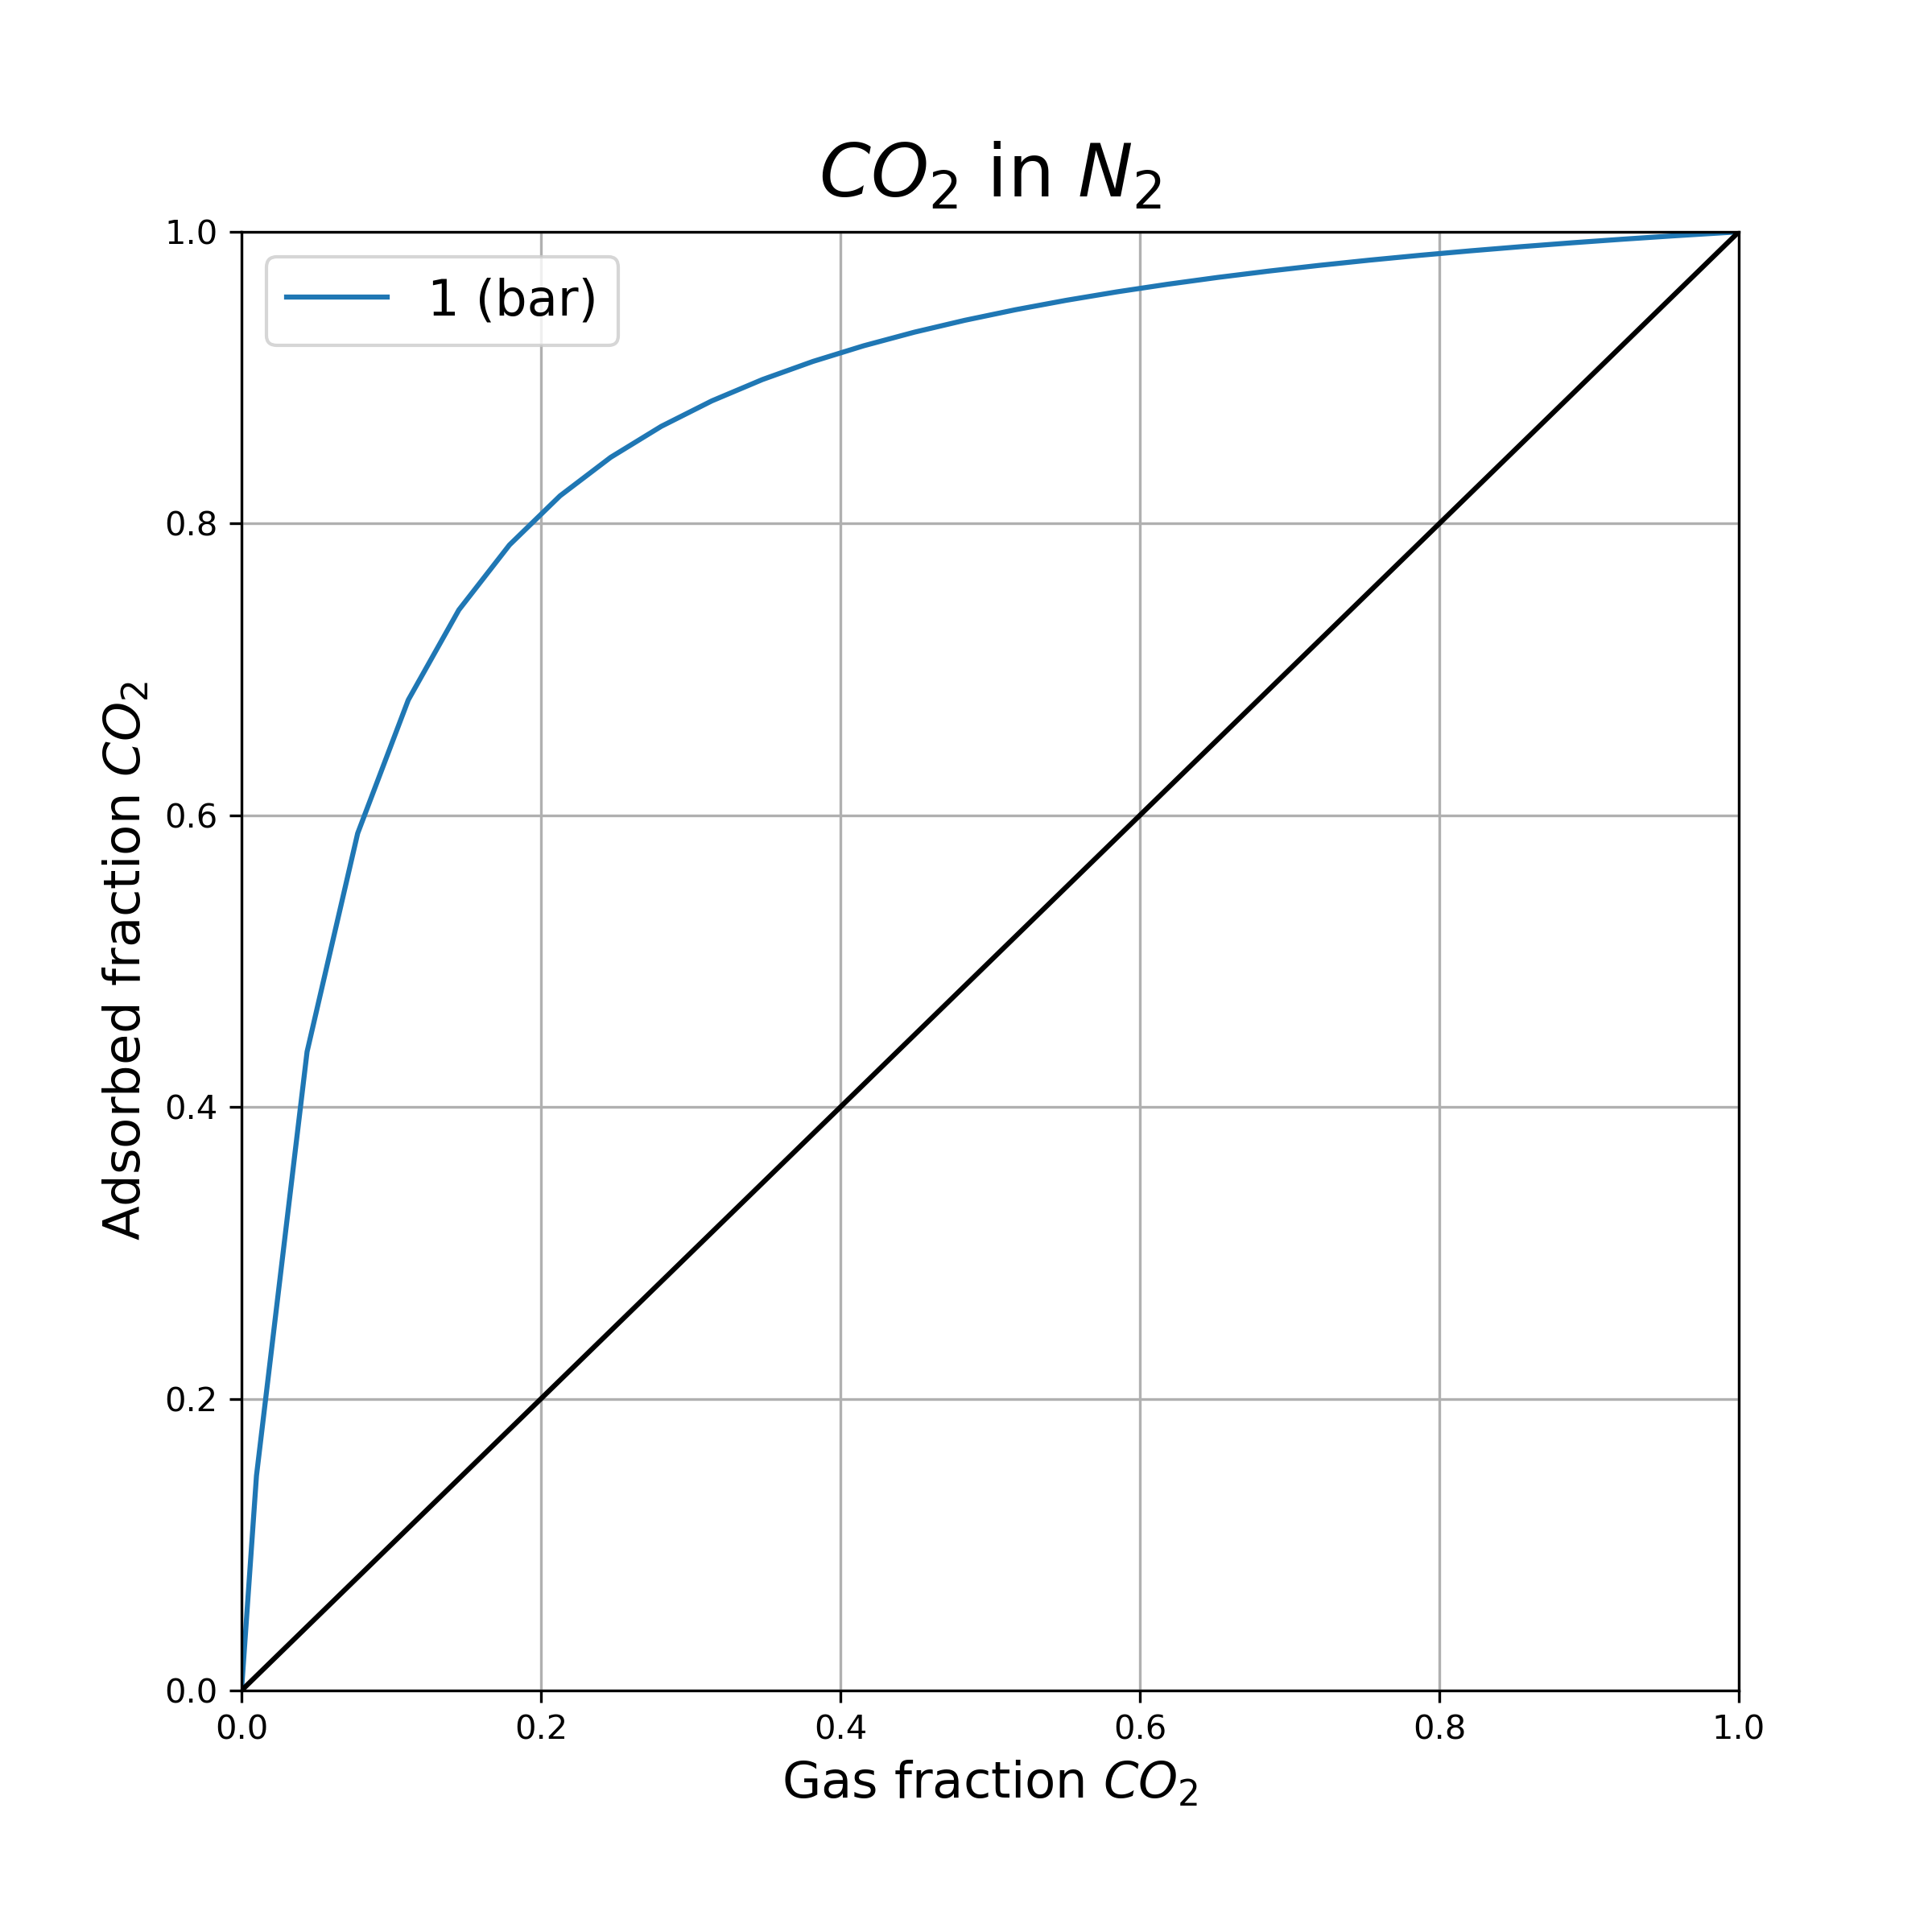
\includegraphics[width=0.92\linewidth]{iast/takeda-co2n2-vle}
        \caption{}%
        \label{pyg:fig:takedaco2n2iast}
    \end{subfigure}
    \caption{
    Modelling binary adsorption of \ce{CO2} and \ce{N2}: 
    (\protect\subref{pyg:fig:takedaco2n2iso}) the pure component
    isotherms and their best fit models and 
    (\protect\subref{pyg:fig:takedaco2n2iast}) 
    the predicted composition of the gaseous
    and adsorbed phase for different fractions of 
    \ce{CO2} at \SI{1}{\bar}
    }%
    \label{pyg:fig:takedaco2n2}

\end{figure}

For the propane-propylene separation, we simulate the selectivity for
propane within a pressure range for a 50\% mixture of the two gases. 
It can be seen that there is little or no preference for the 
unsaturated molecule, though the selectivity increases slightly at 
pressures above \SI{1}{\bar}.

\begin{figure}[htb]

    \centering
    \begin{subfigure}[b]{.45\textwidth}
        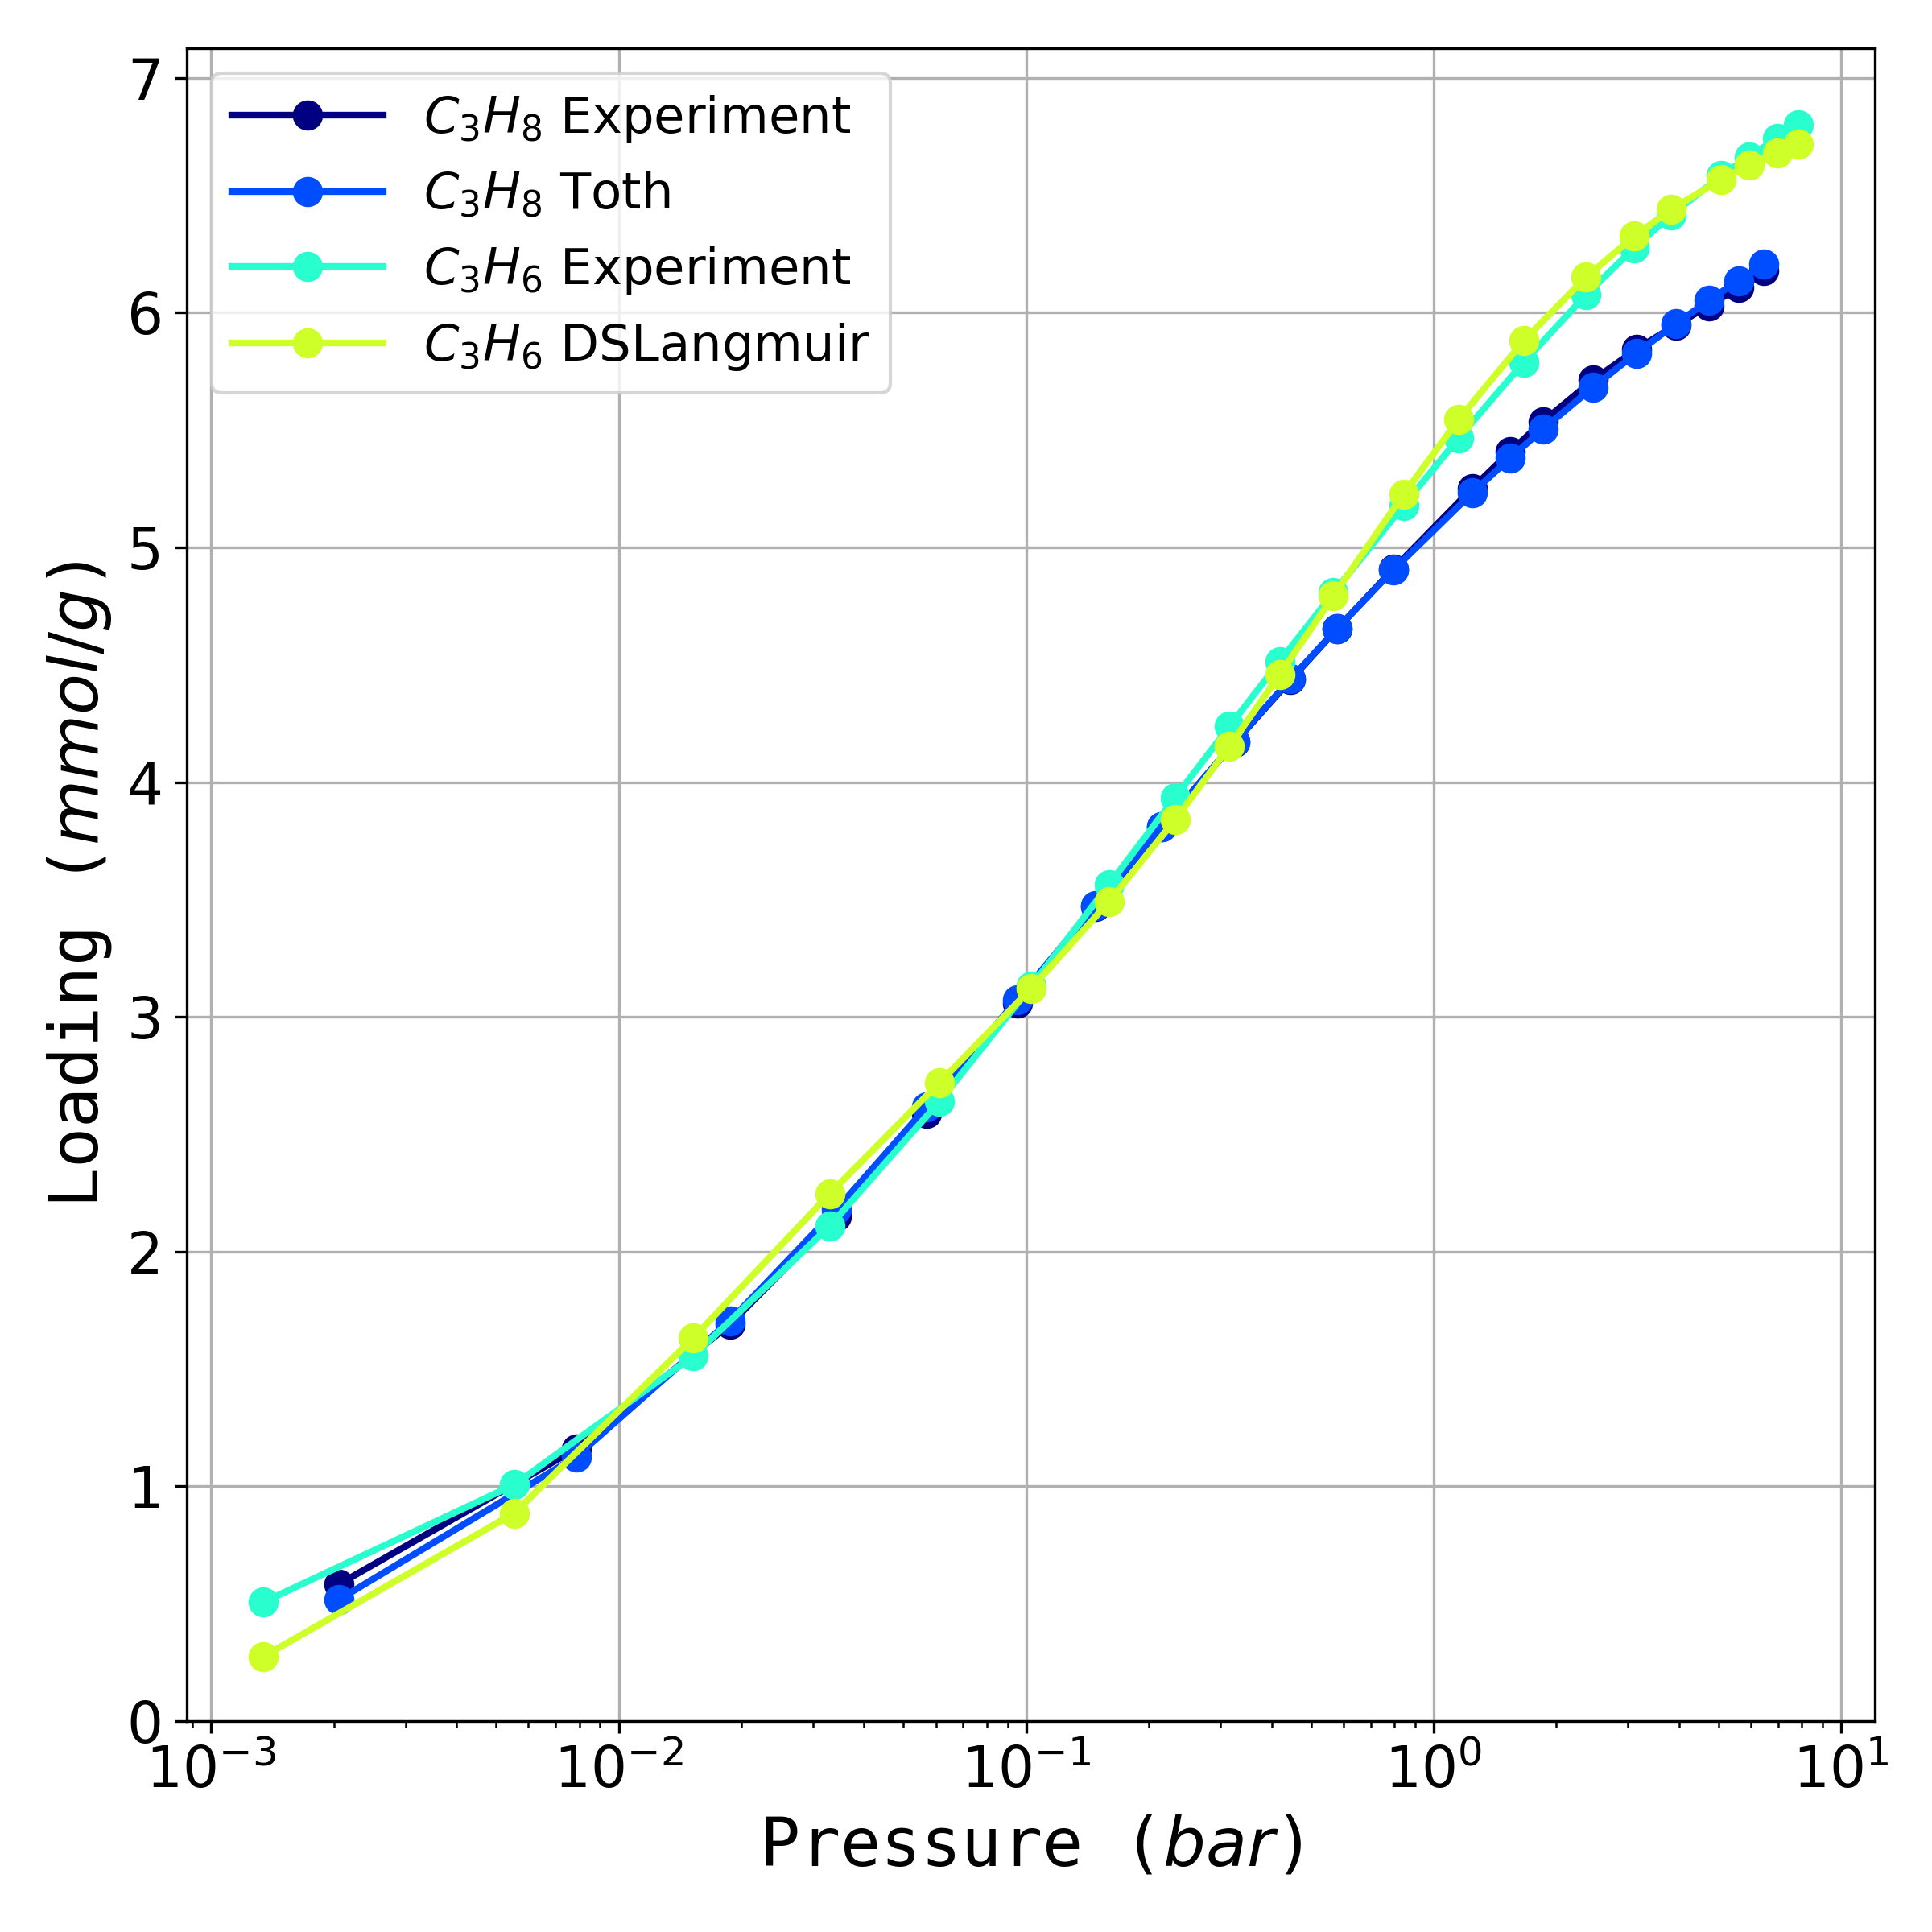
\includegraphics[width=.9\linewidth]{iast/takeda-c3h6c3h8}
        \caption{}%
        \label{pyg:fig:takedac3h6c3h8iso}
    \end{subfigure}
    \begin{subfigure}[b]{.45\textwidth}
        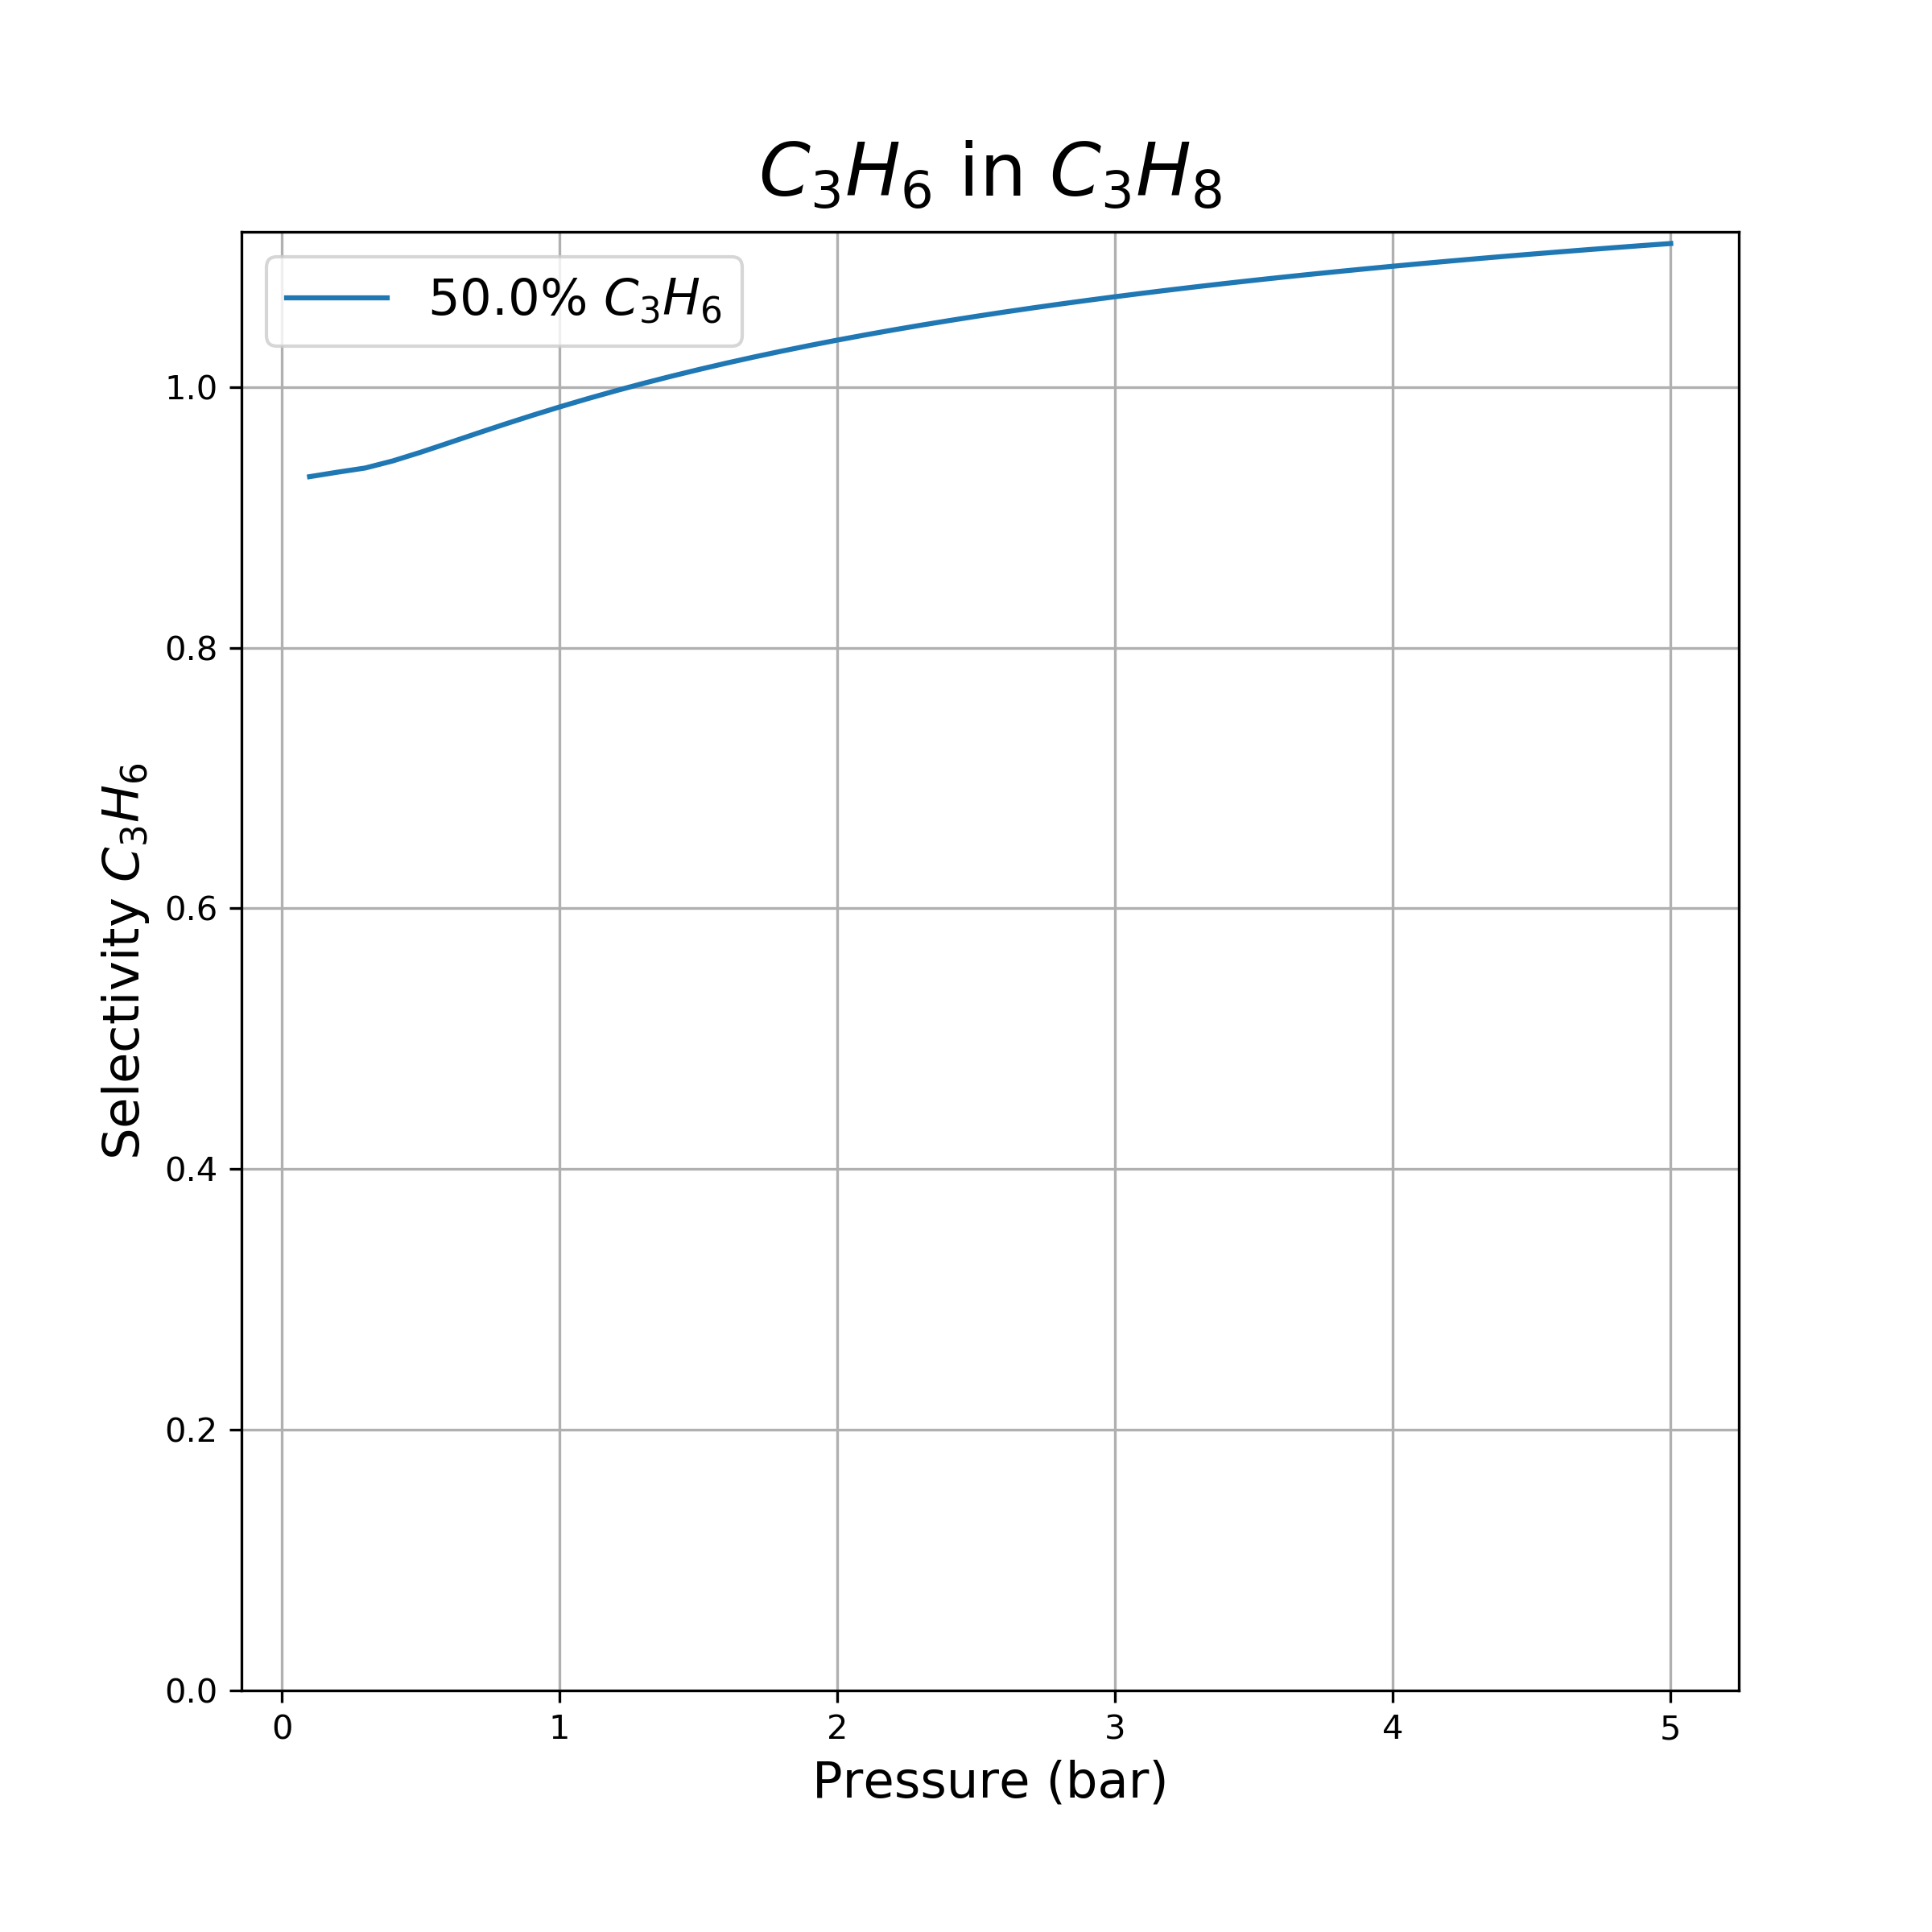
\includegraphics[width=\linewidth]{iast/takeda-c3h6c3h8-svp}
        \caption{}%
        \label{pyg:fig:takedac3h6c3h8iast}
    \end{subfigure}
    \caption{%
    Modelling binary adsorption of a propane-propylene mixture: 
    (\protect\subref{pyg:fig:takedac3h6c3h8iso}) the pure-component
    isotherms and their best fit models and 
    (\protect\subref{pyg:fig:takedac3h6c3h8iast})
    the predicted selectivity of propane adsorption 
    of a 50-50\% mixture in a range of pressure from 0.1 to 7 bar}%
    \label{pyg:fig:takedac3h6c3h8}

\end{figure}